\documentclass[turkish]{eqengconf}
\usepackage[T1]{fontenc}   %%%% PDF Font kodlaması için
\usepackage[utf8]{inputenc}   %%%% Editör font kodlaması için
%\usepackage{showframe}
\usepackage{blindtext} %%% \blindtext komutu için kullanılıyor. Makale bitiminde kaldırılabilir.
\usepackage{wrapfig}  %%% Şekillerin etrafın metini sarmak için kullanılıyor. Yoksa kaldırılabilir.
\usepackage{amsmath}

%%% Optional Math Operation: Makes bold greek letters more bold
\usepackage{upgreek}   %Needed for Matrix Greek Letters
\usepackage{pdfrender} %Needed for Matrix Greek Letters
\newcommand*{\boldgreek}[1]{%
	\textpdfrender{%
		TextRenderingMode=FillStroke,%
		LineWidth=.35pt,%
	}{#1}%
}

\title{BİLDİRİ BAŞLIĞI BİLDİRİ BAŞLIĞI BİLDİRİ BAŞLIĞI\\
	BİLDİRİ BAŞLIĞI BİLDİRİ BAŞLIĞI BİLDİRİ BAŞLIĞI}
\author{\authorname{1}{Ahmet Yılmaz},
		\authorname{*}{Hakan Özen} ve
		\authorname{1}{John Doe}}

\date{%%% \date kullanılarak, kurum ve e-posta bilgileri girilmektedir.
	\affils{1}{Araş. Gör., İnşaat Müh. Bölümü, Abece Üniversitesi, Güzelkent}\\
	\affils{*}{Prof. Dr., Jeofizik Müh. Bölümü, Abece Teknik Üniversitesi, Büyükkent}\\
	\email{gönderenyazar@kurum.edu.tr}%%% Sadece gönderen yazarın e-postası girilecektir.
}

%%% Turkish Support


%%% BibLatex
\usepackage[]{babel}
\usepackage{xkeyval}
\usepackage[style=authoryear,maxcitenames=2,maxbibnames=10, 
doi=false,isbn=false,url=false,eprint=false,giveninits]{biblatex}
\usepackage{etoolbox}
\usepackage[style=english]{csquotes}

%%%%% TURKISH NOTATION FOR BIBLATEX. TURN OFF FOR ENGLISH %%%%%
\DefineBibliographyStrings{english}{%
	references = {KAYNAKLAR},
	and = {ve},
	andothers = {vd.},
	pages = {s.},
	mathesis = {Yüksek Lisans Tezi},
	phdthesis = {Doktora Tezi},
	techreport = {Teknik Rapor},}
%%%%%%%%%%%%%%%%%%%%%%%%%%%%%%%%%%%%%%%%%%%%%%%%%%%

%%%%% ENGLISH NOTATION FOR BIBLATEX. TURN OFF FOR TURKISH %%%%%
%\DefineBibliographyStrings{english}{%
%	mathesis = {M.S. Thesis},}
%%%%%%%%%%%%%%%%%%%%%%%%%%%%%%%%%%%%%%%%%%%%%%%%%%%

\renewbibmacro{in:}{}
\DeclareNameAlias{sortname}{family-given}
\DeclareFieldFormat[article]{number}{\mkbibparens{#1}}
\DeclareFieldFormat[article]{volume}{\mkbibbold{#1}}
\DeclareFieldFormat[article]{journaltitle}{\mkbibemph{#1}\addcomma}
\DeclareFieldFormat[article]{title}{\mkbibquote{#1\addcomma}}
\DeclareFieldFormat[thesis]{title}{\mkbibemph{#1}}

\renewbibmacro*{volume+number+eid}{%
	\printfield{volume}%
	%  \setunit*{\adddot}% DELETED
	\setunit*{\addnbthinspace}% \addnbthinspace or \addnbspace
	\printfield{number}%
	\setunit{\addcomma\space}%
	\printfield{eid}}

\addbibresource{examplebib.bib}

\begin{document}

%%%%%% Keep thes lines %%%%%
\fixturkishbug %% For the Turkish-\includegraphics bug
\maketitle
\thispagestyle{firststyle}
%%%%%%%

 
%%% A Turkish Abstract has to be provided if the paper is in Turkish
\begin{ozeteq}
\blindtext
\end{ozeteq}

\begin{anahtarkelimeler}
anahtar kelime1, anahtar kelime2, anahtar kelime3.
\end{anahtarkelimeler}


%%% All papers (both Turkish and English) have to provide English Title and Abstract

\titlesecondary{TITLE OF THE PAPER TITLE OF THE PAPER\\TITLE OF THE PAPER TITLE OF THE PAPER}

\begin{abstracteq} 
\blindtext
\end{abstracteq}

\begin{keywords}
keyword1, keyword2, keyword3.
\end{keywords}

 
\section{GİRİŞ BÖLÜMÜ}
\blindtext
\begin{equation}\label{eq:massdef}    %Denklemden önce boşluk bırakılmamalı
x=\dfrac{a}{b}, \quad \boldgreek{\alpha}=\boldgreek{\upphi}
\end{equation}

\blindtext

Görüldüğü üzere, sonuçların doğru olduğu anlaşılmaktadır. Hatalı sonuçlar için başka yorumların yapılması uygun olacaktır (\cite{Skinner1993}).

\section{TEORİ BÖLÜMÜ}

\blindtext

\subsection{Denklemler}
\blindtext
\begin{equation}\label{eq:energy} %Denklemden önce boşluk bırakılmamalı
g(x)=\int_a^b f(x)dx, \quad x=\dfrac{a}{b}, \quad \boldgreek{\alpha}=\boldgreek{\upphi}
\end{equation}

Denklem (\ref{eq:energy})'de de görüldüğü üzere, sonuçların doğru olduğu 
anlaşılmaktadır. Hatalı sonuçlar için başka yorumların yapılması uygun 
olacaktır. \textcite{Narasimhan2006, Erkus2006}'da gösterildiği üzere, yapılan 
çalışmaların uygun olduğu anlaşılmaktadır. \cite{Bekin2018-MSThesis}, 
\cite{Constantinou2011}.

\blindtext

\subsection{Diğer Bilgiler}
\blindtext

Şekil (\ref{fig:structure})'de de görüldüğü üzere, sonuçların doğru olduğu anlaşılmaktadır. Hatalı sonuçlar için başka yorumların yapılması uygun olacaktır.

\blindtext

\begin{wrapfigure}{r}{0.4\textwidth}
	\vspace{-12pt}
	\centering
	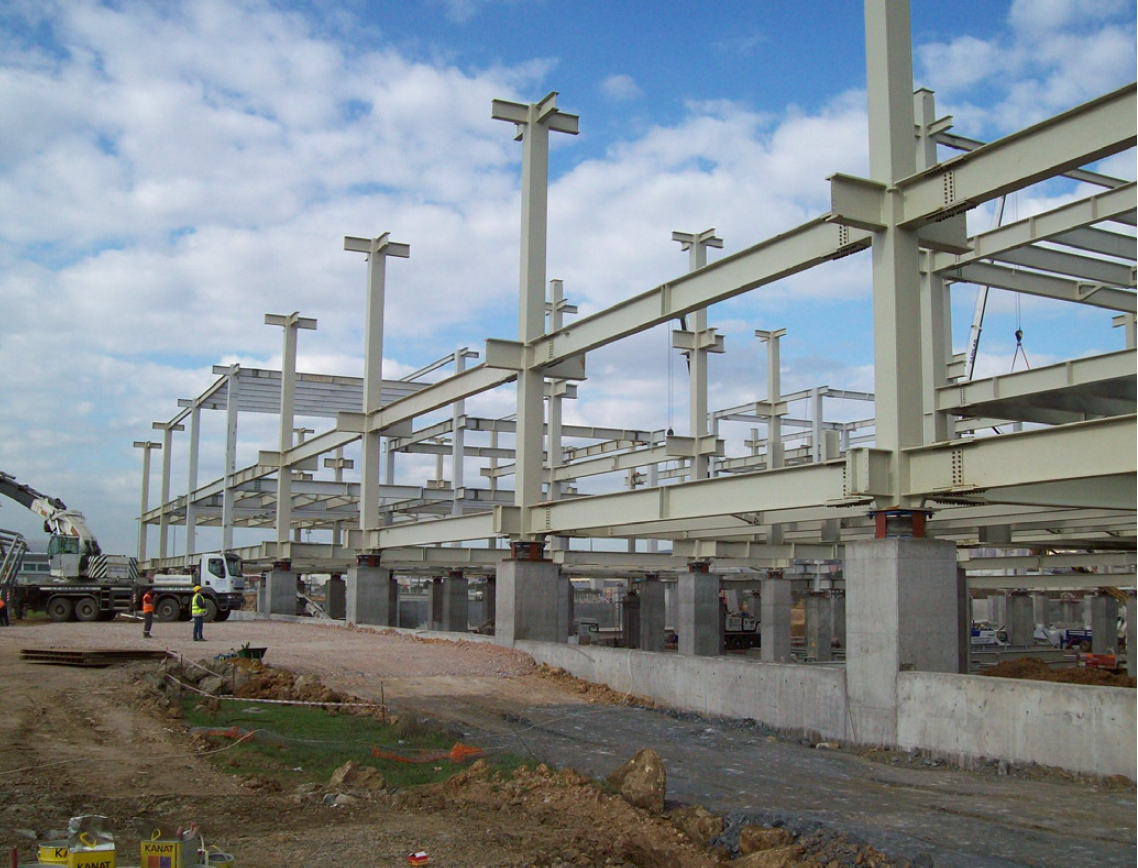
\includegraphics[scale=0.2]{b.PNG}
	\caption{\label{fig:structure}Bir bina yapısı.}
	\vspace{-10pt}
\end{wrapfigure}

\blindtext

Şekil (\ref{fig:otherstruct})'de de görüldüğü üzere, sonuçların doğru olduğu anlaşılmaktadır. Hatalı sonuçlar için başka yorumların yapılması uygun olacaktır.

\begin{figure}[]
	\centering
	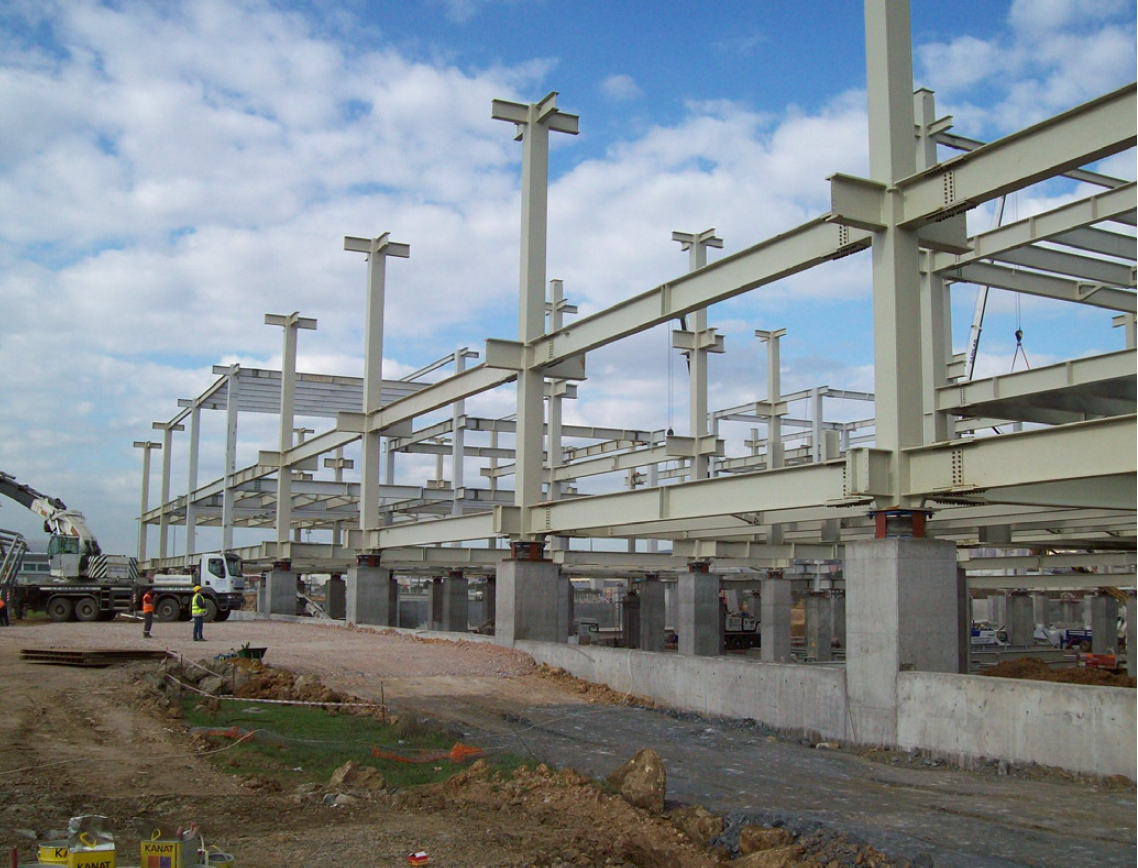
\includegraphics[scale=0.4]{b.PNG}
	\caption{\label{fig:otherstruct}Diğer bina.}
\end{figure}

\blindtext
\begin{equation}\label{eq:stiffness} %Denklemden önce boşluk bırakılmamalı
g(x)=\int_a^b f(x)dx, \quad x=\dfrac{a}{b}, \quad \boldgreek{\alpha}=\boldgreek{\upphi}
\end{equation}

Denklem (\ref{eq:stiffness})'de de görüldüğü üzere, sonuçların doğru olduğu anlaşılmaktadır. Hatalı sonuçlar için başka yorumların yapılması uygun olacaktır.

\blindtext

\subsubsection*{Alt Alt Başlık}
\blindtext

\blindtext

\subsection{Başka Diğer Bilgiler}
\blindtext

\blindtext


\begin{table}[]
%	\vspace{-5pt}
	\setlength\abovecaptionskip{-5pt}
	\setlength\belowcaptionskip{10pt}
	\centering
		\caption{\label{tab:onemlibilgi}Önemli Bilgiler.}
		\begin{tabular}{l|c|r} % <-- Alignments: 1st column left, 2nd middle and 3rd right, with vertical lines in between
			\textbf{Value 1} & \textbf{Value 2} & \textbf{Value 3}\\
			$\alpha$ & $\beta$ & $\gamma$ \\
			\hline
			1 & 1110.1 & a\\
			2 & 10.1 & b\\
			3 & 23.113231 & c\\
		\end{tabular}
\end{table}

Tablo (\ref{tab:onemlibilgi})'de de görüldüğü üzere, sonuçların doğru olduğu anlaşılmaktadır. Hatalı sonuçlar için başka yorumların yapılması uygun olacaktır.

\blindtext

\blindtext

\section{YENİ BÖLÜM}
\blindtext

\blindtext

\subsection{Başka Diğer Bilgiler}

\blindtext

\subsection{Başka Başka Diğer Bilgiler}

\blindtext

\begin{wraptable}{l}{6cm}
	\setlength\abovecaptionskip{0pt}
	\setlength\belowcaptionskip{15pt}
	\vspace{-10pt}
	\centering
	\caption{\label{tab:baskasonuc}Başka sonuçlar.}
	\begin{tabular}{l|c|r} % <-- Alignments: 1st column left, 2nd middle and 3rd right, with vertical lines in between
		\textbf{Value 1} & \textbf{Value 2} & \textbf{Value 3}\\
		$\alpha$ & $\beta$ & $\gamma$ \\
		\hline
		1 & 1110.1 & a\\
		2 & 10.1 & b\\
		3 & 23.113231 & c\\
	\end{tabular}
    \vspace{-10pt}
\end{wraptable}

Tablo (\ref{tab:baskasonuc})'de de görüldüğü üzere, sonuçların doğru olduğu anlaşılmaktadır. Hatalı sonuçlar için başka yorumların yapılması uygun olacaktır.

\blindtext

\subsubsection*{Alt Alt Başlık}
\blindtext

\blindtext

\subsection{Başka Diğer Bilgiler}
\blindtext

\blindtext

\begin{figure}[h]
	\centering
	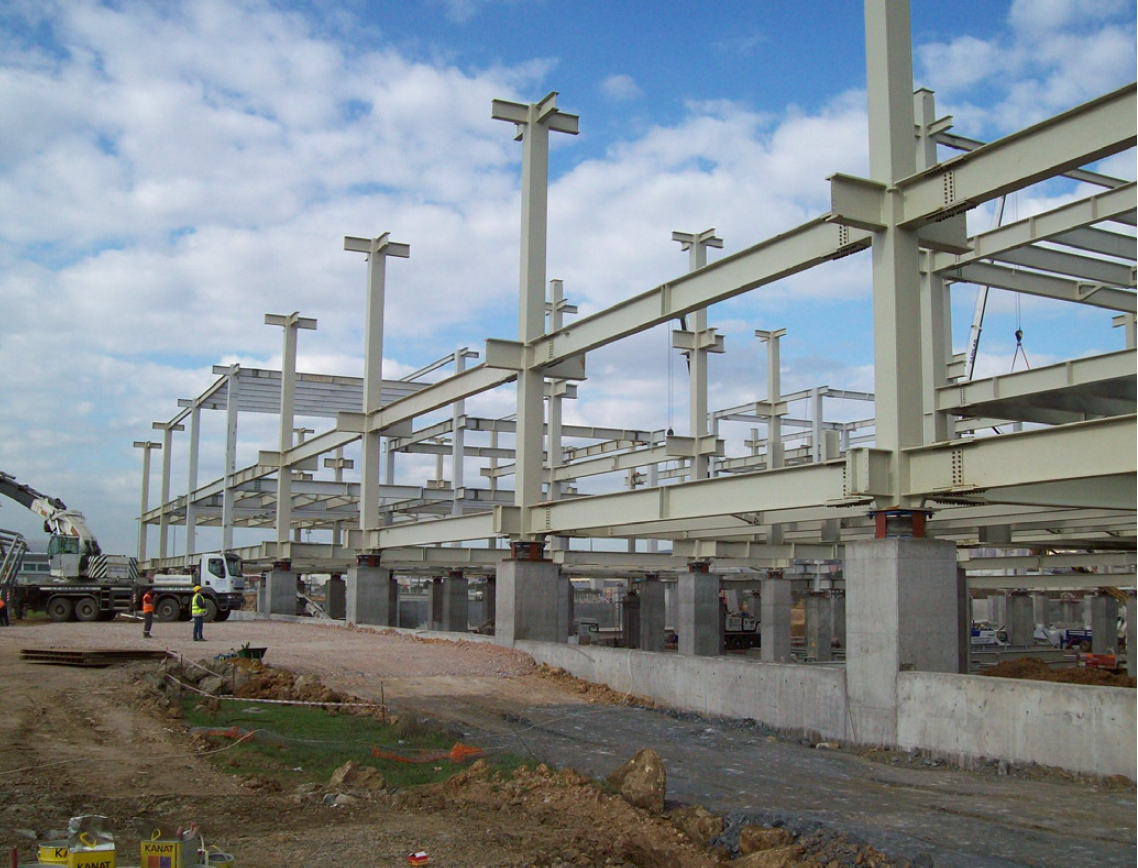
\includegraphics[scale=0.4]{b.PNG}
	\caption{\label{fig:ikinciyapi} Başka başka şekiller.}
\end{figure}

Şekil (\ref{fig:ikinciyapi})'de de görüldüğü üzere, sonuçların doğru olduğu anlaşılmaktadır. Hatalı sonuçlar için başka yorumların yapılması uygun olacaktır.

\blindtext

\section{SONUÇ}
\blindtext

\blindtext

\printbibliography

\end{document}